\chapter{Hiện thực và kiểm thử}
\section{Hiện thực}

Mô tả quá trình triển khai hệ thống học tập sử dụng LLMs (Large Language Models) để sinh ra các bài học đề xuất cho sinh viên dựa trên các bài học có sẵn từ giảng viên. Hệ thống được xây dựng trên nền tảng frontend sử dụng VueJS với Vuetify và Tailwind để phát triển giao diện người dùng, và backend được phát triển bằng FastAPI với kiến trúc DDD (Domain-Driven Design) và sử dụng PostgreSQL làm cơ sở dữ liệu.

\subsection{Kiến trúc hệ thống}

Hệ thống được chia thành hai phần chính: frontend và backend.

\subsubsection{Frontend (VueJS với Vuetify và Tailwind)}

Giao diện người dùng được xây dựng với VueJS để tạo ra các trang web động, hỗ trợ các tính năng như: dashboard, course list, course detail, feedback, và giao diện nhập mục tiêu học (goal input). Vuetify được sử dụng để phát triển các component UI, đảm bảo tính thẩm mỹ và khả năng sử dụng cao. Tailwind CSS được sử dụng để tùy chỉnh giao diện và tạo kiểu cho các thành phần UI một cách linh hoạt và dễ dàng. Mỗi trang và chức năng được thiết kế đơn giản và dễ sử dụng, bao gồm các mục như: lời chào, hoạt động gần đây, phản hồi và danh sách các khóa học mà sinh viên đang tham gia.

\subsubsection{Backend (FastAPI với DDD architecture)}

FastAPI được chọn làm framework backend nhờ vào khả năng xử lý nhanh và hỗ trợ RESTful API. Kiến trúc DDD (Domain-Driven Design) được áp dụng để chia hệ thống thành các domain riêng biệt như: Users, Courses, Lessons, Feedback, và Learning Outcomes. Điều này giúp mã nguồn dễ duy trì, mở rộng và dễ hiểu. PostgreSQL được sử dụng để lưu trữ dữ liệu về các khóa học, lessons, learning outcomes, feedback từ sinh viên, và các mục tiêu học của sinh viên. Mỗi học phần (lesson) của khóa học được lưu trong cơ sở dữ liệu, cùng với các thông tin về mục tiêu học và phản hồi từ sinh viên.

\subsection{Quá trình triển khai}

\subsubsection{Tạo cấu trúc cơ sở dữ liệu}

Các bảng cơ sở dữ liệu được thiết kế để lưu trữ các thông tin về khóa học, lessons, các bài học (modules), feedback của sinh viên, và các mục tiêu học. Mỗi bảng liên quan đến các thực thể trong hệ thống được cấu hình phù hợp với yêu cầu của DDD. Các bảng liên quan đến sinh viên và giảng viên cũng được liên kết để theo dõi các hoạt động học tập của sinh viên.

\subsubsection{Xây dựng các API}

Các API cho phép sinh viên và giảng viên tương tác với hệ thống, bao gồm việc đăng nhập, xem danh sách khóa học, xem chi tiết khóa học, gửi feedback, và nhập mục tiêu học. Backend của hệ thống sử dụng FastAPI để xử lý các yêu cầu HTTP nhanh chóng, đảm bảo hiệu suất và khả năng mở rộng.

\begin{figure}[H]
    \centering
    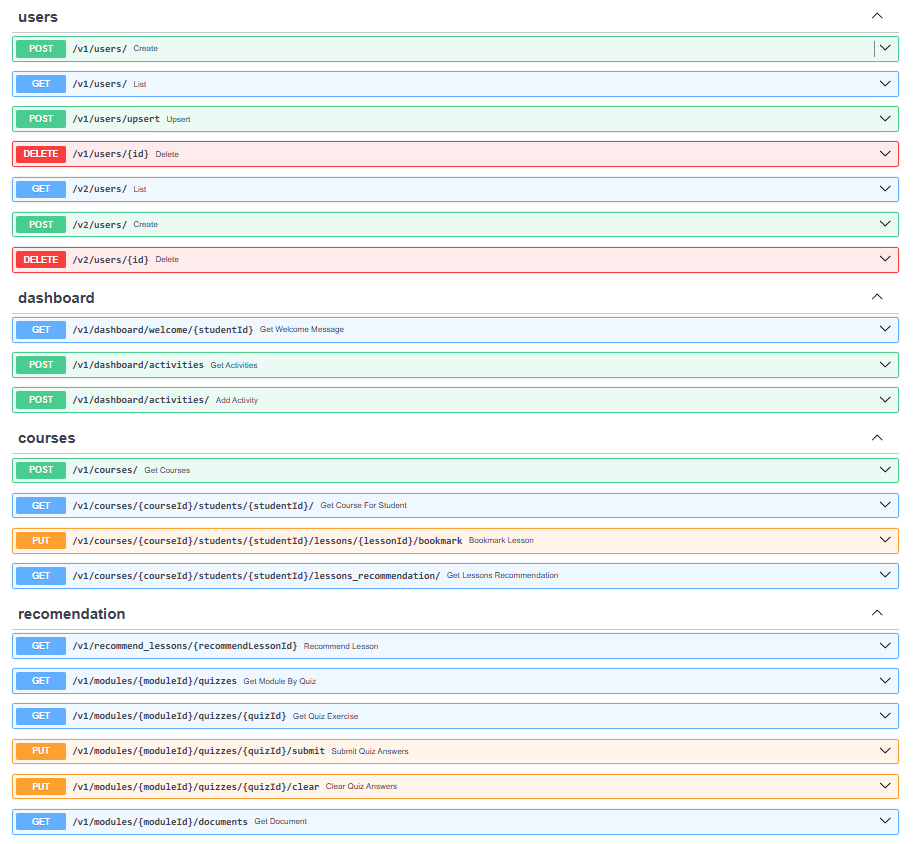
\includegraphics[width=0.8\textwidth]{Images/Implement/APIs.png}
    \caption{API endpoints}
\end{figure}
\subsubsection{Quản lý bài học và đề xuất học tập}

Giảng viên có thể đăng các khóa học cùng với learning outcomes và lessons. Hệ thống sẽ sử dụng LLMs để phân tích mục tiêu học của sinh viên và tự động đề xuất các lessons phù hợp, dựa trên nội dung và mục tiêu học của giảng viên đã đăng. Mỗi lesson sẽ bao gồm các module (quiz, code exercises, reading materials). LLMs sẽ được tích hợp vào backend để tự động tạo nội dung học cho sinh viên. Khi sinh viên nhập mục tiêu học, hệ thống sẽ phân tích mục tiêu và so sánh với các learning outcomes đã có của giảng viên để đề xuất bài học phù hợp.

\subsubsection{Giao diện người dùng}

VueJS và Vuetify tạo ra một giao diện người dùng dễ sử dụng và thân thiện. Trang dashboard của sinh viên hiển thị thông tin về các khóa học đang học, thông báo về các hoạt động gần đây, và phần gửi feedback cho hệ thống. Các sinh viên có thể nhập mục tiêu học vào một modal trong trang Course Detail để hệ thống đề xuất lessons và modules phù hợp với mục tiêu của họ. Hệ thống cũng ghi lại thời gian học của sinh viên để theo dõi tiến độ học tập và tạo ra các báo cáo cho lộ trình học tập tiếp theo.

\section{Kiểm thử}

\subsection{Tổng quan về kiểm thử}

Mục đích của kiểm thử trong hệ thống: Đảm bảo rằng các tính năng hoạt động đúng, hệ thống không có lỗi và có thể chịu được tải trong quá trình sử dụng thực tế.

\subsubsection{Loại kiểm thử thực hiện:}
\begin{itemize}
    \item \textbf{Kiểm thử chức năng:} Đảm bảo các chức năng của hệ thống (đăng nhập, nhập mục tiêu học, gửi feedback, xem course details, v.v.) hoạt động đúng.
    \item \textbf{Kiểm thử hiệu suất:} Đảm bảo hệ thống có thể xử lý nhiều yêu cầu đồng thời và không gặp phải vấn đề về hiệu suất.
    \item \textbf{Kiểm thử bảo mật:} Đảm bảo hệ thống bảo vệ tốt các dữ liệu người dùng và tránh các tấn công bảo mật (ví dụ: SQL Injection, Cross-site Scripting).
    \item \textbf{Kiểm thử tích hợp:} Kiểm tra sự hoạt động đồng bộ của các module frontend và backend.
    \item \textbf{Kiểm thử hồi quy:} Đảm bảo những thay đổi mới không làm hỏng các tính năng cũ của hệ thống.
\end{itemize}

\subsection{Kiểm thử API}

\subsubsection{Kịch bản Kiểm thử}

\subsubsubsection{1. Kiểm thử API Chào mừng (Welcome API)}

\textbf{Mục đích:} Kiểm thử khả năng lấy thông báo chào mừng cho sinh viên qua API GET /v1/dashboard/welcome/{studentId}.

\textbf{Test Case 1: Lấy thông báo chào mừng với Student ID hợp lệ}
\begin{itemize}
    \item \textbf{Mô tả:} Gửi yêu cầu GET đến API /v1/dashboard/welcome/{studentId} với Student ID hợp lệ.
    \item \textbf{Kết quả mong đợi:}
    \begin{itemize}
        \item Mã phản hồi là 200.
        \item Trường isSuccess có giá trị true.
        \item Trường message là chuỗi ký tự.
        \item Trường data chứa các thông tin về khóa học, course\_id, và last\_accessed.
    \end{itemize}
\end{itemize}

\textbf{Test Case 2: Lấy thông báo chào mừng với Student ID không hợp lệ}
\begin{itemize}
    \item \textbf{Mô tả:} Gửi yêu cầu GET đến API /v1/dashboard/welcome/{studentId} với Student ID không hợp lệ.
    \item \textbf{Kết quả mong đợi:}
    \begin{itemize}
        \item Mã phản hồi là 500.
        \item Thông báo lỗi chỉ ra việc kiểm tra không thành công.
    \end{itemize}
\end{itemize}

\subsubsubsection{2. Kiểm thử API Lấy Hoạt động (Get Activities API)}

\textbf{Mục đích:} Kiểm thử khả năng lấy danh sách hoạt động của sinh viên qua API POST /v1/dashboard/activities.

\textbf{Test Case 1: Lấy danh sách hoạt động với phân trang mặc định}
\begin{itemize}
    \item \textbf{Mô tả:} Gửi yêu cầu POST đến API /v1/dashboard/activities với Student ID hợp lệ và tham số phân trang mặc định (limit: 0, offset: 0).
    \item \textbf{Kết quả mong đợi:}
    \begin{itemize}
        \item Mã phản hồi là 200.
        \item Trường isSuccess có giá trị true.
        \item Trả về danh sách hoạt động với các trường như activity\_id, activity\_description, activity\_type, activity\_date.
    \end{itemize}
\end{itemize}

\textbf{Test Case 2: Lấy danh sách hoạt động với giới hạn tùy chỉnh}
\begin{itemize}
    \item \textbf{Mô tả:} Gửi yêu cầu POST với Student ID hợp lệ và tham số phân trang (limit: 5, offset: 0).
    \item \textbf{Kết quả mong đợi:}
    \begin{itemize}
        \item Trả về tối đa 5 hoạt động.
        \item Phân trang đúng.
    \end{itemize}
\end{itemize}

\textbf{Test Case 3: Lấy danh sách hoạt động với offset}
\begin{itemize}
    \item \textbf{Mô tả:} Gửi yêu cầu POST với Student ID hợp lệ và tham số phân trang (limit: 10, offset: 10).
    \item \textbf{Kết quả mong đợi:}
    \begin{itemize}
        \item Trả về hoạt động từ bản ghi thứ 11.
        \item Phân trang đúng.
    \end{itemize}
\end{itemize}

\textbf{Test Case 4: Lấy danh sách hoạt động với Student ID không hợp lệ}
\begin{itemize}
    \item \textbf{Mô tả:} Gửi yêu cầu POST với Student ID không hợp lệ.
    \item \textbf{Kết quả mong đợi:}
    \begin{itemize}
        \item Mã phản hồi là 500.
        \item Lỗi xác thực chi tiết.
    \end{itemize}
\end{itemize}

\subsubsubsection{3. Kiểm thử API Lấy Danh sách Khóa học (Courses List API)}

\textbf{Mục đích:} Kiểm thử khả năng lấy danh sách khóa học cho sinh viên qua API POST /v1/courses/.

\textbf{Test Case 1: Lấy danh sách khóa học với phân trang mặc định}
\begin{itemize}
    \item \textbf{Mô tả:} Gửi yêu cầu POST với Student ID hợp lệ và tham số phân trang mặc định (offset: 0, page\_size: 10).
    \item \textbf{Kết quả mong đợi:}
    \begin{itemize}
        \item Mã phản hồi là 200.
        \item Trả về danh sách các khóa học với các thông tin chi tiết như id, name, start\_date, end\_date, student\_list, learning\_outcomes.
    \end{itemize}
\end{itemize}

\textbf{Test Case 2: Lấy danh sách khóa học với kích thước trang tùy chỉnh}
\begin{itemize}
    \item \textbf{Mô tả:} Gửi yêu cầu POST với Student ID hợp lệ và tham số phân trang (offset: 0, page\_size: 20).
    \item \textbf{Kết quả mong đợi:}
    \begin{itemize}
        \item Trả về tối đa 20 khóa học.
        \item Phân trang đúng.
    \end{itemize}
\end{itemize}

\textbf{Test Case 3: Lấy danh sách khóa học với offset lớn}
\begin{itemize}
    \item \textbf{Mô tả:} Gửi yêu cầu POST với Student ID hợp lệ và tham số phân trang (offset: 100, page\_size: 10).
    \item \textbf{Kết quả mong đợi:}
    \begin{itemize}
        \item Trả về phản hồi hợp lý.
        \item Hệ thống xử lý tốt với các offset lớn.
    \end{itemize}
\end{itemize}

\textbf{Test Case 4: Lấy danh sách khóa học với Student ID không hợp lệ}
\begin{itemize}
    \item \textbf{Mô tả:} Gửi yêu cầu POST với Student ID không hợp lệ.
    \item \textbf{Kết quả mong đợi:}
    \begin{itemize}
        \item Mã phản hồi là 500.
        \item Lỗi xác thực chi tiết.
    \end{itemize}
\end{itemize}

\subsubsubsection{4. Kiểm thử API Lấy Chi tiết Khóa học (Get Course for Student API)}

\textbf{Mục đích:} Kiểm thử khả năng lấy chi tiết khóa học cho sinh viên qua API GET /v1/courses/{courseId}/students/{studentId}/.

\textbf{Test Case 1: Lấy chi tiết khóa học với ID hợp lệ}
\begin{itemize}
    \item \textbf{Mô tả:} Gửi yêu cầu GET với courseId và studentId hợp lệ.
    \item \textbf{Kết quả mong đợi:}
    \begin{itemize}
        \item Mã phản hồi là 200.
        \item Trường isSuccess có giá trị true.
        \item Trả về các thông tin chi tiết khóa học như course\_id, student\_id, completed\_lessons, time\_spent, assignments\_done, và các bài học liên quan.
    \end{itemize}
\end{itemize}

\textbf{Test Case 2: Lấy chi tiết khóa học với Student ID không khớp với Course ID}
\begin{itemize}
    \item \textbf{Mô tả:} Gửi yêu cầu GET với courseId hợp lệ và studentId không khớp.
    \item \textbf{Kết quả mong đợi:} Hệ thống trả về lỗi thích hợp với thông báo lỗi nhất quán.
\end{itemize}

\textbf{Test Case 3: Lấy chi tiết khóa học với ID không hợp lệ}
\begin{itemize}
    \item \textbf{Mô tả:} Gửi yêu cầu GET với courseId và studentId không hợp lệ.
    \item \textbf{Kết quả mong đợi:}
    \begin{itemize}
        \item Mã phản hồi là 422.
        \item Lỗi xác thực chi tiết.
    \end{itemize}
\end{itemize}

\subsubsubsection{5. Kiểm thử API Lấy Danh sách Khóa học Đề xuất (Recommended Courses List API)}

\textbf{Mục đích:} Kiểm thử khả năng lấy danh sách khóa học đề xuất cho sinh viên qua API GET /{courseId}/students/{studentId}/lessons\_recommendation/.

\textbf{Test Case 1: Lấy danh sách khóa học với phân trang mặc định}
\begin{itemize}
    \item \textbf{Mô tả:} Gửi yêu cầu GET với student\_id và course\_id hợp lệ.
    \item \textbf{Kết quả mong đợi:}
    \begin{itemize}
        \item Mã phản hồi là 200.
        \item Trả về danh sách khóa học với các chi tiết như course\_id, course\_name, lesson\_id, bookmark, status, title, description.
    \end{itemize}
\end{itemize}

\textbf{Test Case 2: Lấy danh sách khóa học với Course ID không hợp lệ}
\begin{itemize}
    \item \textbf{Mô tả:} Gửi yêu cầu GET với student\_id hợp lệ và course\_id không hợp lệ.
    \item \textbf{Kết quả mong đợi:}
    \begin{itemize}
        \item Mã phản hồi là 500.
        \item Lỗi xác thực chi tiết.
    \end{itemize}
\end{itemize}

\textbf{Test Case 3: Lấy danh sách khóa học với Student ID không hợp lệ}
\begin{itemize}
    \item \textbf{Mô tả:} Gửi yêu cầu GET với student\_id không hợp lệ.
    \item \textbf{Kết quả mong đợi:}
    \begin{itemize}
        \item Mã phản hồi là 500.
        \item Lỗi xác thực chi tiết.
    \end{itemize}
\end{itemize}

\subsubsubsection{6. Kiểm thử API Thêm Hoạt động (Add Activity API)}

\textbf{Mục đích:} Kiểm thử khả năng thêm hoạt động cho sinh viên qua API POST /activities/.

\textbf{Test Case 1: Thêm hoạt động hợp lệ}
\begin{itemize}
    \item \textbf{Mô tả:} Gửi yêu cầu POST với dữ liệu hợp lệ (bao gồm student\_id, type, description).
    \item \textbf{Kết quả mong đợi:}
    \begin{itemize}
        \item Trạng thái trả về là 200 với thông điệp "Successfully added the activity."
    \end{itemize}
\end{itemize}

\textbf{Test Case 2: Thêm hoạt động thiếu student\_id}
\begin{itemize}
    \item \textbf{Mô tả:} Gửi yêu cầu POST mà không có trường student\_id.
    \item \textbf{Kết quả mong đợi:}
    \begin{itemize}
        \item Mã phản hồi là 400.
        \item Lỗi xác thực chi tiết.
    \end{itemize}
\end{itemize}


\subsubsection{Kết quả kiểm thử API}
